\chapter{Project evaluation}

\epigraph{Yeah you wanted a hit \\ but tell me \\ where's the point in it?}{You Wanted a Hit \\ LCD Soundsystem, 2010}

\section{Digital release}

This thesis project lives on 2 different repositories, hosted on GitHub, to foster collaboration via \glspl{issue} and \glspl{pull-request}, and also with frequent updates, to show people the whole process behind this thesis project.

The main repository contains this thesis document, Jupyter notebooks for machine learning, documentation for beginners and educators, and auxiliary shell scripts. It is hosted at \url{https://github.com/montoyamoraga/tiny-trainable-instruments}.

The auxiliary repository contains the Arduino library, including its source code and examples. It is hosted at \url{https://github.com/montoyamoraga/TinyTrainable}.

\section{Workshop}

As a way of user testing and releasing this thesis, some workshops were conducted during TODO, with support from a grant at CAMIT for teaching the workshops in English in USA, and in Chile in Spanish, remotely over teleconferencing software and after being approved by the MIT COUHES TODO explain.


\begin{figure}[ht]
  \centering
  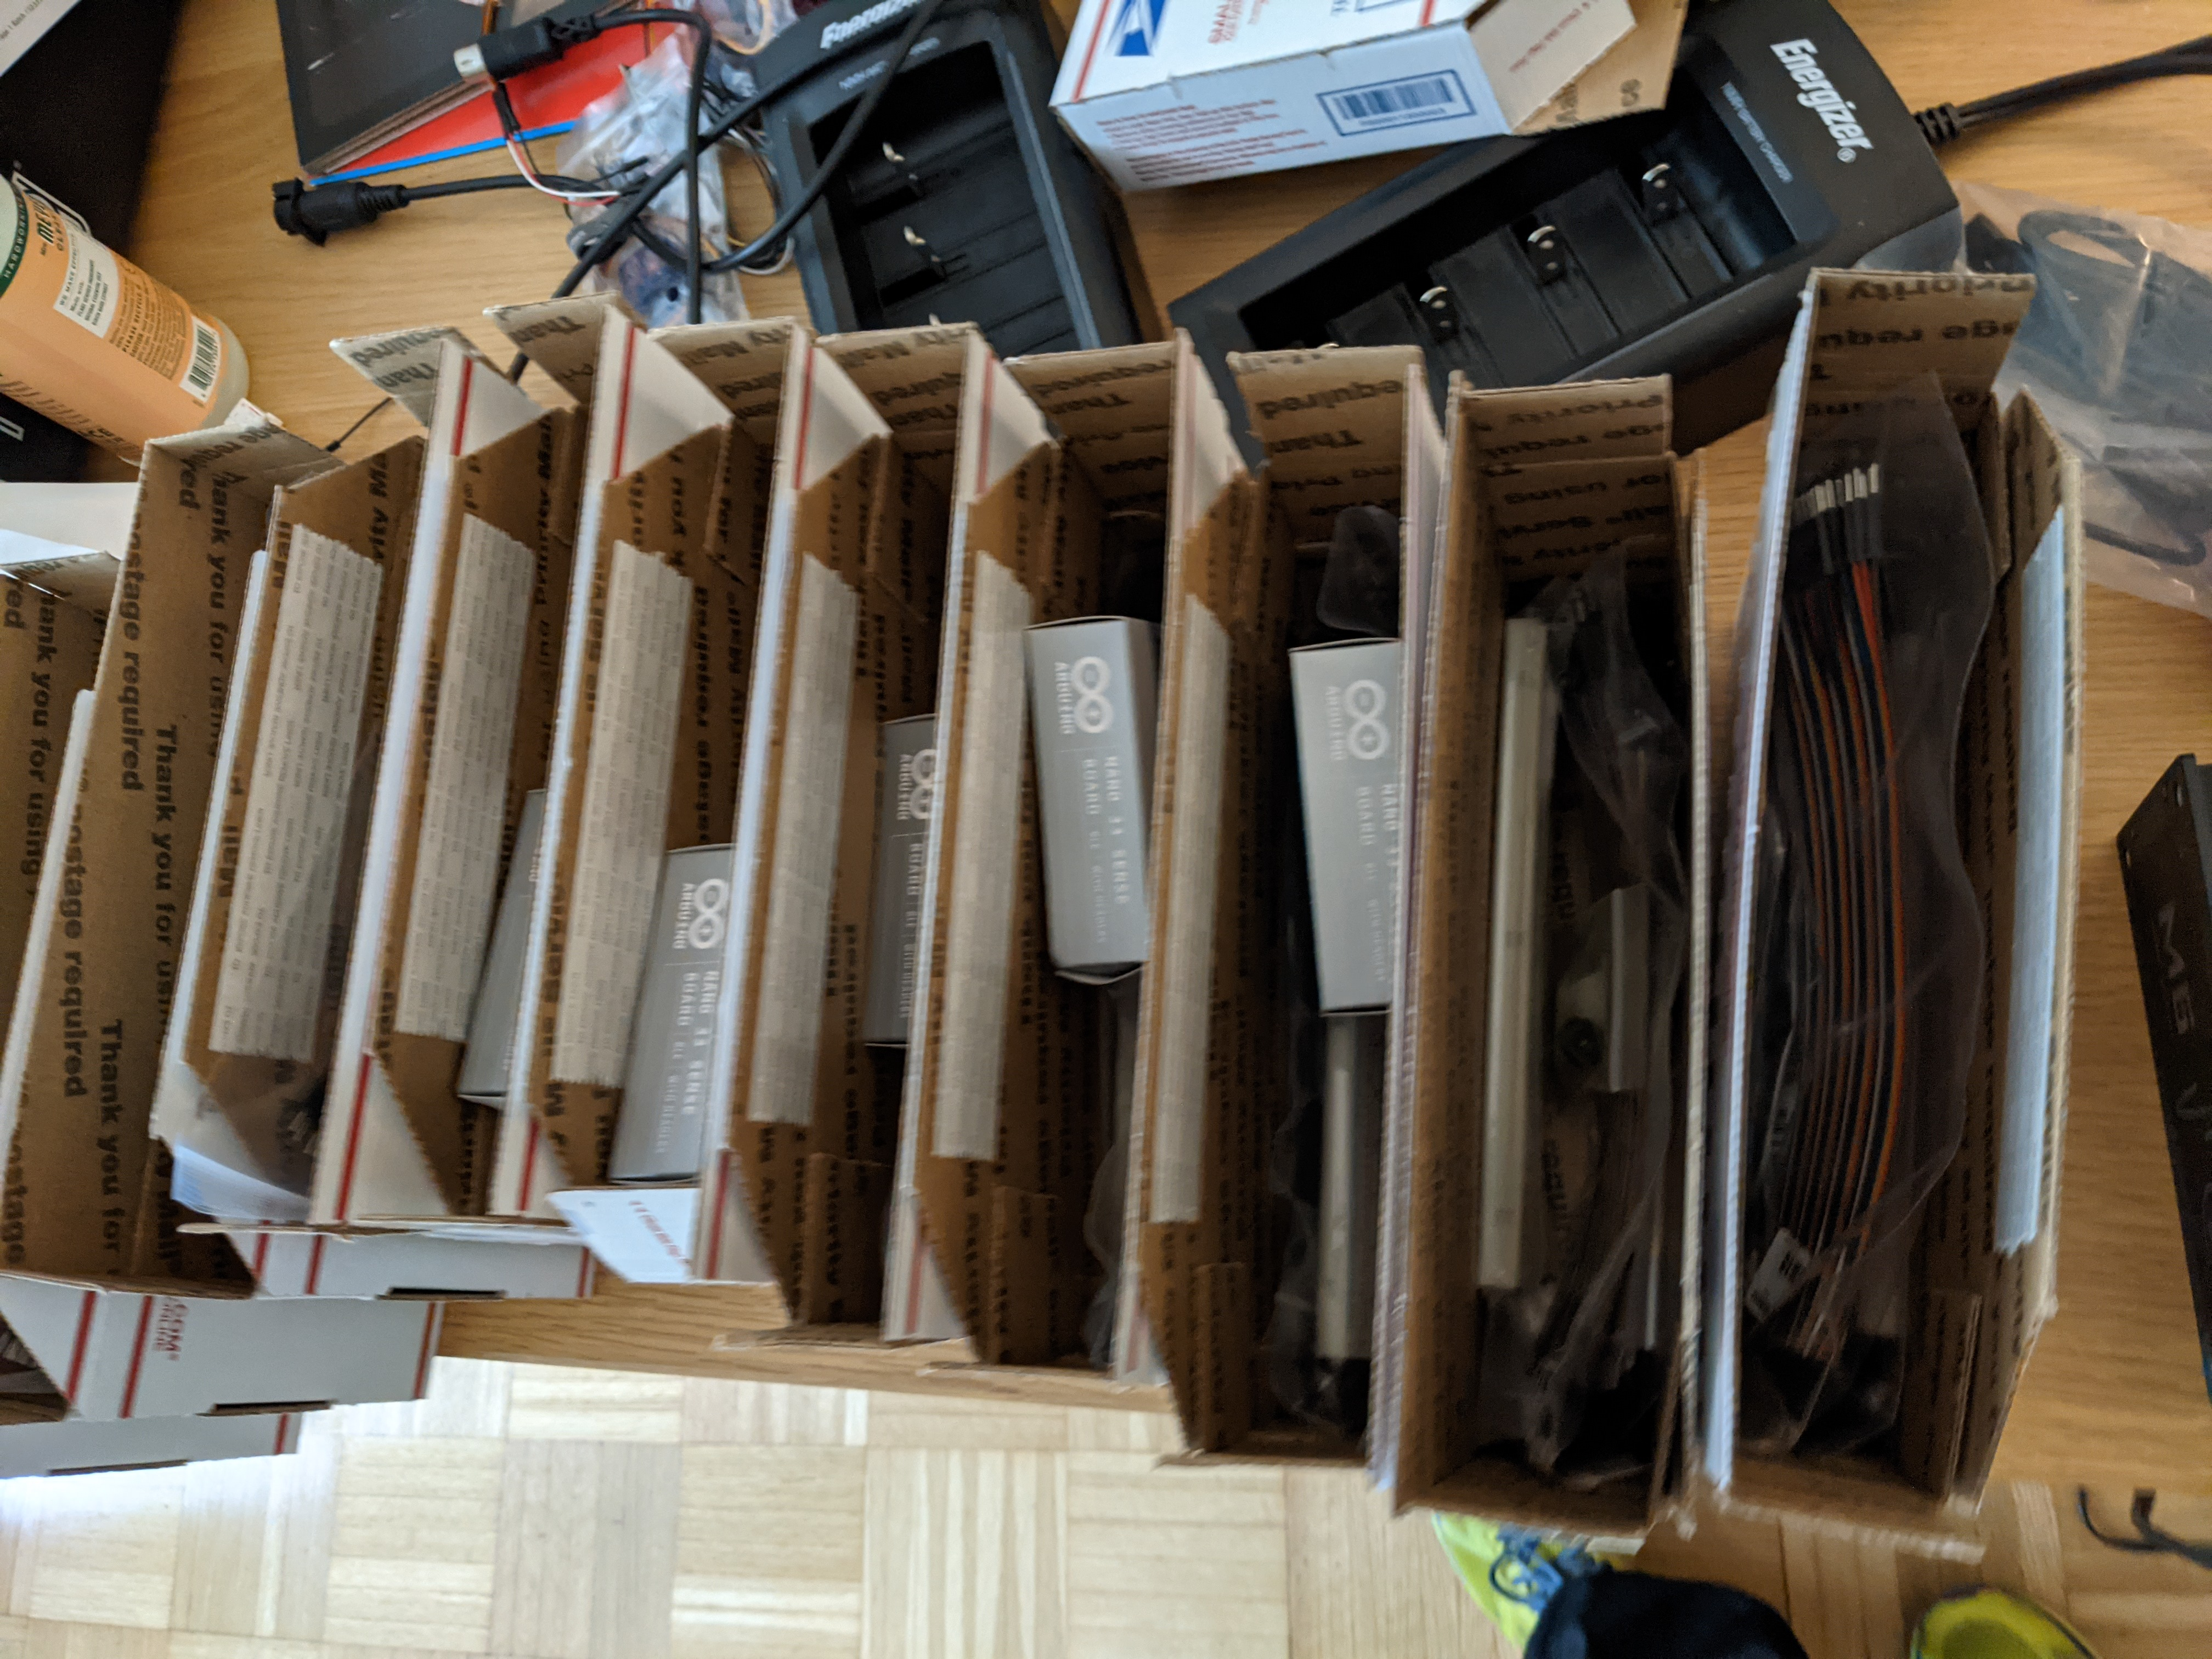
\includegraphics[width=0.75\linewidth,height=0.25\textheight,keepaspectratio]{images/workshop-packages.jpg}
  \caption{Workshop packages}
  \caption*{Picture by myself}
  \label{fig:workshop-packages}
\end{figure}


The workshop instructions are documented on the docs/ folder of the repository available at \url{https://github.com/montoyamoraga/tiny-trainable-instruments}

Each workshop consists of 2 sessions of 2 hours each, spread over 2 consecutive days.

In the first session we will first help people with installation of the software, and then move on to start wiring the materials on the electronic breadboard material. We will concentrate on the simpler examples with color input. We will also collect data of gesture and speech to create custom databases and use them to train other slow machine learning models that will keep on running on the student's workshops after the workshop is over.

In the second session we will use the result of the trained models to create more advanced instruments that react to gesture and speech. We will also show the participants the other 

I applied to and was awarded a grant by the Council for the arts at MIT (CAMIT), which consisted of 2,000.00 USD to buy materials to teach the Tiny Trainable Instruments workshop to 20 people, during June 2021.

I taught this workshop 3 times, 2 of them were in English for people based in the USA, and 1 time in Spanish for people based in Chile, with a total of 20 kits being delivered.

\begin{figure}[ht]
  \centering
  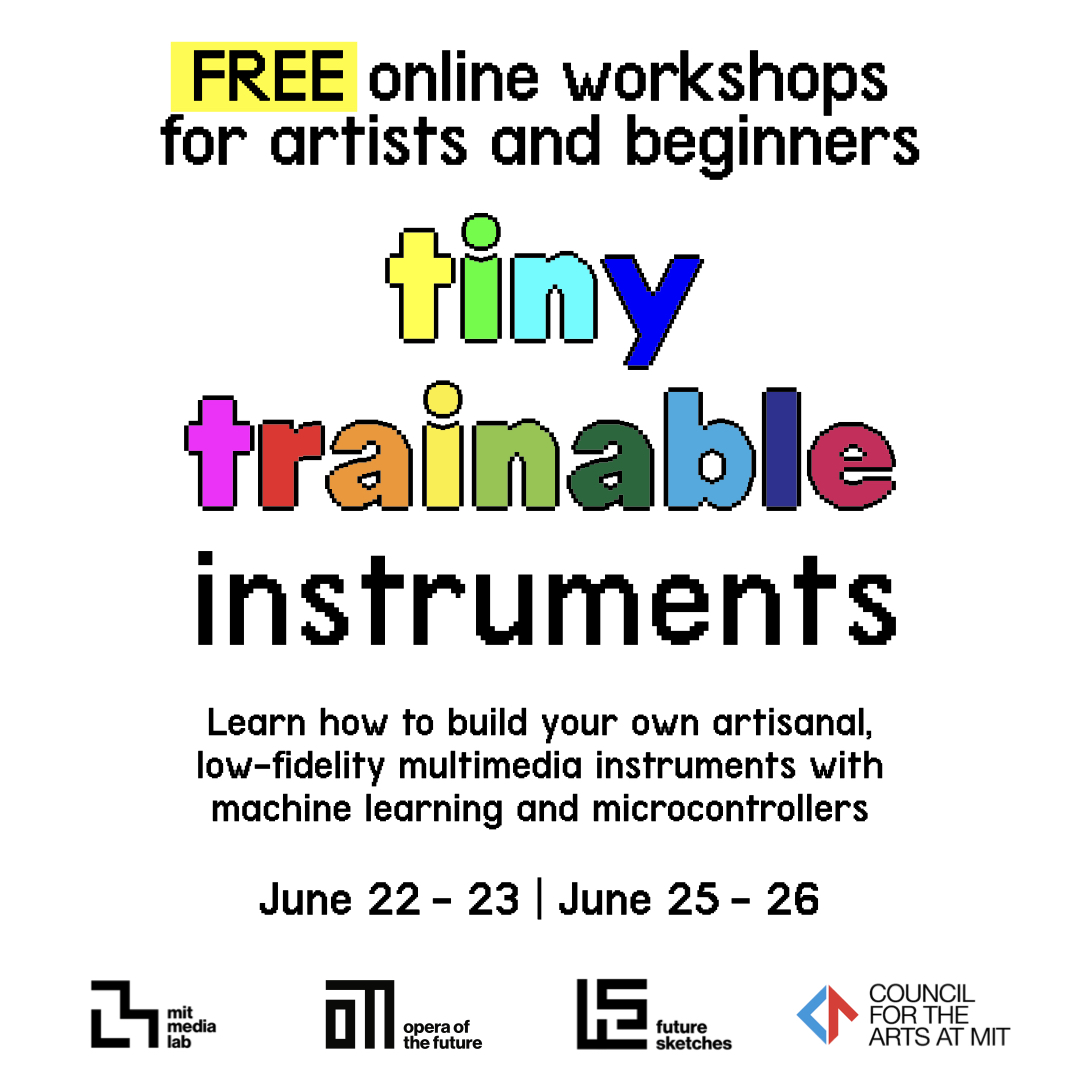
\includegraphics[width=0.75\linewidth,height=0.35\textheight,keepaspectratio]{images/workshop-en-1.jpg}
  \caption{Workshop flyer cover in English}
  \caption*{Graphics by Renata Gaui}
  \label{fig:workshop-english-flyer-page-1}
\end{figure}

\begin{figure}[ht]
  \centering
  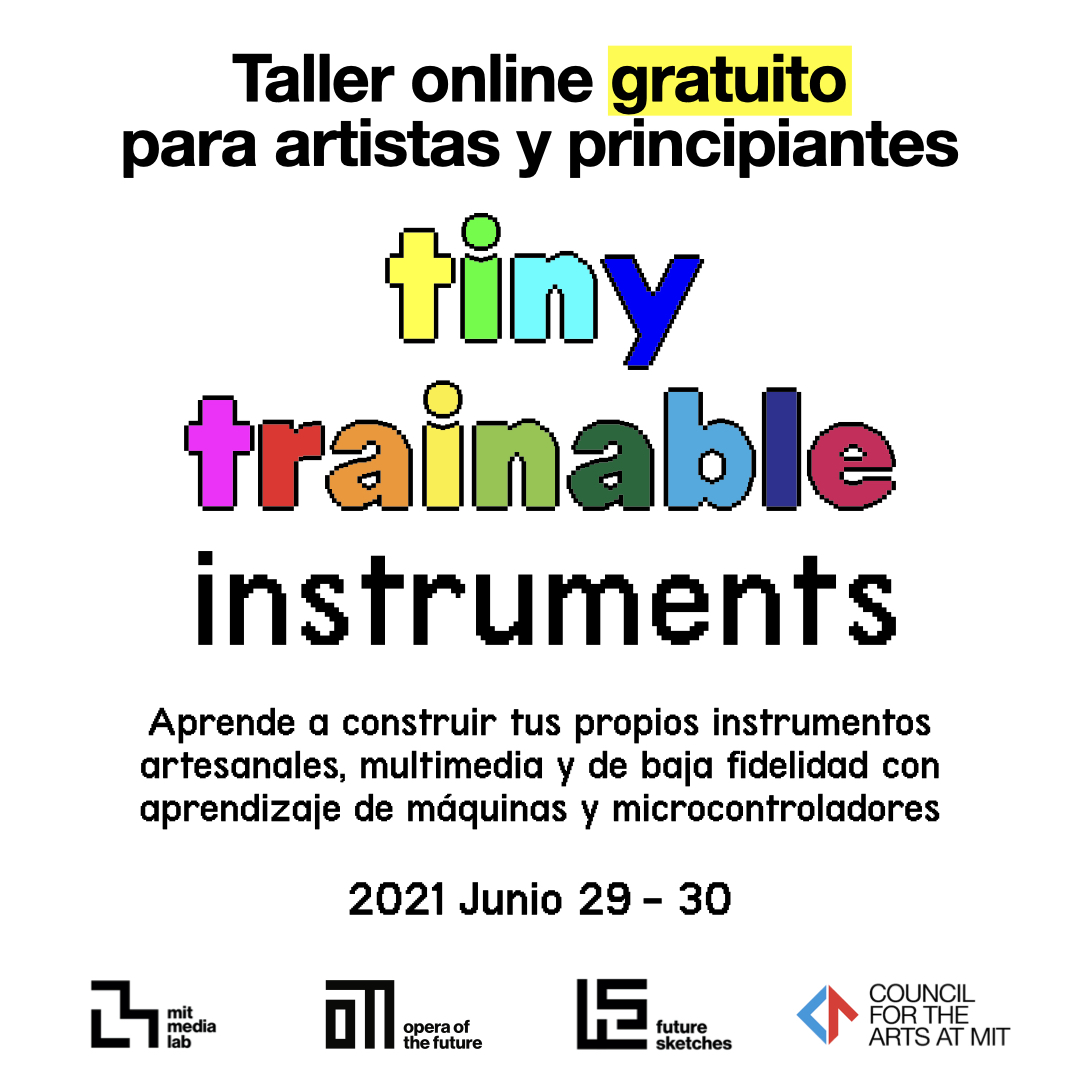
\includegraphics[width=0.75\linewidth,height=0.35\textheight,keepaspectratio]{images/workshop-es-1.jpg}
  \caption{Workshop flyer cover in Spanish}
  \caption*{Graphics by Renata Gaui}
  \label{fig:workshop-spanish-flyer-page-1}
\end{figure}

The multimedia aspect of this project was featured, in particular the ability to use different inputs, including color, gesture and speech, to control different outputs, including serial messages, sound, and motor movement.

\begin{figure}[ht]
  \centering
  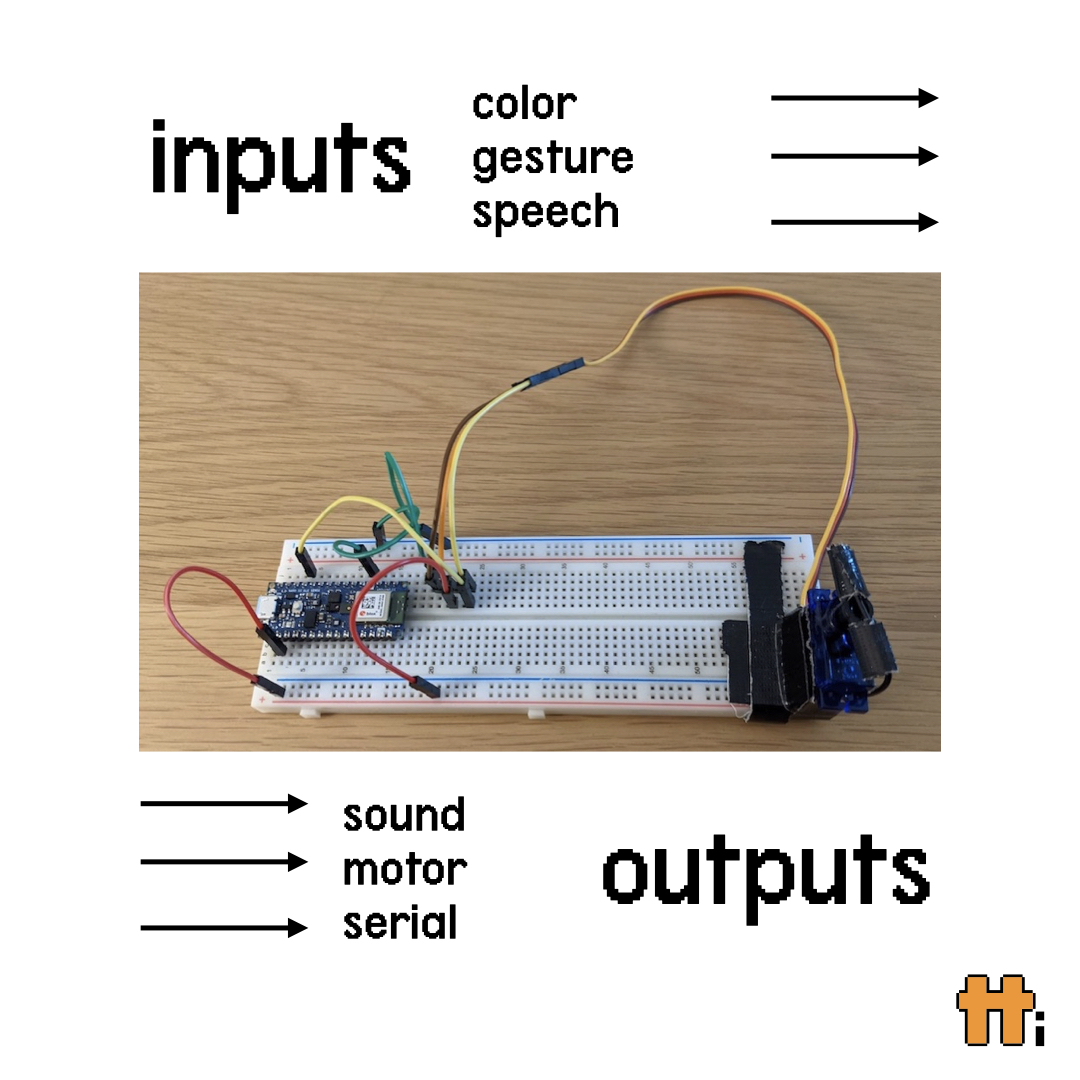
\includegraphics[width=0.75\linewidth,height=0.35\textheight,keepaspectratio]{images/workshop-en-2.jpg}
  \caption{Workshop multimedia output in English}
  \caption*{By Renata Gaui}
  \label{fig:workshop-english-flyer-page-2}
\end{figure}

\begin{figure}[ht]
  \centering
  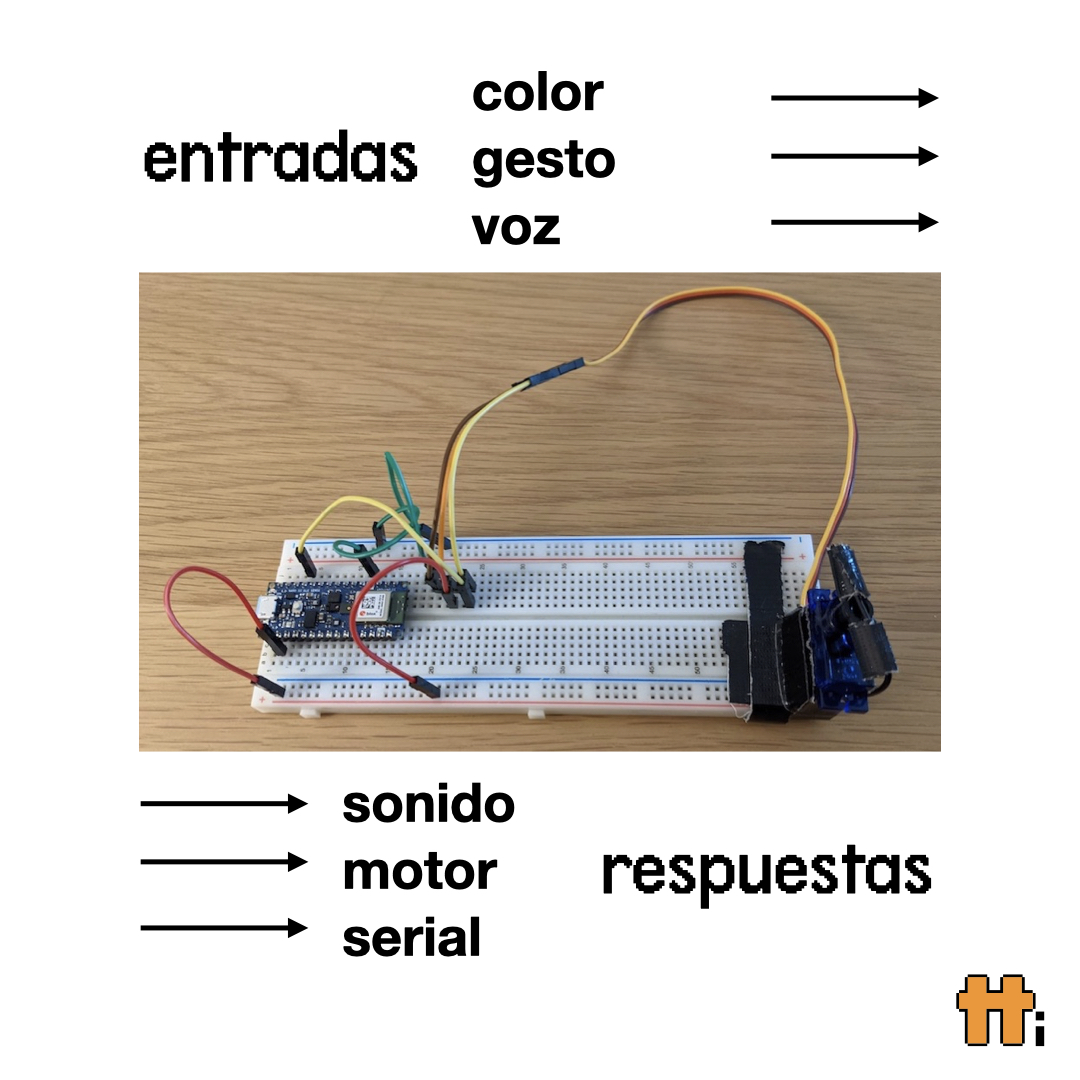
\includegraphics[width=0.75\linewidth,height=0.35\textheight,keepaspectratio]{images/workshop-es-2.jpg}
  \caption{Workshop multimedia output in Spanish}
  \caption*{By Renata Gaui}
  \label{fig:workshop-spanish-flyer-page-2}
\end{figure}

\section{Multimedia documentation}

TODO: upload a collection of examples made by people who came to the workshops, featuring the software library and what they learned.
